%THEORY
\chapter{Theory}
\label{chapter:theory}
% Innledning
XML is designed for encapsulation of structured and semistructured data,
relational data, and object repositories. The XQuery query language is designed
to perform flexible queries in such data. A translation of the language into
relational algebra requires detailed knowledge about XQuery for a proper translation to be made. In this chapter, section
\ref{sect:theory:xquery} describes important details about the XQuery
language that are essential to this task. Further, existing implementations of
such translators are documented and compared.

Additionally, the concept of classic relational algebra itself is outlined in
section \ref{sect:theory:relAlg}, as the target algebra will be based on much
of its semantics.

Then in section \ref{sect:parser_and_syntaxtrees}, some common strategies for
parsing and construction of parsers are outlined, as well as techniques for
parsing syntax trees.

Finally, a thoroughly researched method for translating XQuery to relational
algebra dubbed ``Loop Lifting'' is described in section \ref{sect:theory:loop_lifting}.

\section{XQuery}

XQuery is a query language developed by the XML Query working group of W3C.
Version 1.0\cite{w3c00} became a W3C Recommendation January 2007. It was designed as a
response to an emerging task: to intelligently express queries in theincreasing
amounts of information stored, exchanged and presented using XML. The language
is derived from Quilt\cite{quilt_queryLanguage}.


\begin{itemize}
\item itroduksjon
\item historie
\item bruksomr\aa der
\item ...
\item atomic vs sequence
\end{itemize}

\subsection{Basics}
\begin{itemize}
  \item sekvenser og ting atomisk, alt je
  \item andre ting som er basisk og ikke surt
\end{itemize}

\subsection{Path Expressions}
\begin{itemize}
\item fra XPath / brukt i mange andre ting (XSLT yeye)
\item ...
\item akser
\item predikat
\item semantikk 
\item eksikveringsorden etc
\end{itemize}

\subsection{FLWOR}

\begin{itemize}
\item motiv
\item ...
\item F L W O R semantikk
\item \^{} --- eksikveringsorden etc
\end{itemize}

\subsection{Binary Operators}

\begin{itemize}
\item motiv
\item ...
\item semantikk
\item hva er sant, hva er usant?
\end{itemize}



\subsection{Evt andre ting fra XQuery vi kommer til \aa~implementere}

\begin{itemize}
\item if then else

\end{itemize}

\subsection{Full Text Extensions}

\begin{itemize}
\item motiv
\item ...
\item semantikk
\item hva har man? ftcontains er kilden...
\end{itemize}
% State of the art, nåværende teknologi og implementasjoner
\section{Current state of XQuery}
\underline{\textbf{\LARGE //TODO:}} Kapittelet m\aa~fylles ut og omstruktureres

There exist a number of XQuery implementations, few however are extended with full text capabilities. This section will briefly present some of the more prominent alternatives.
\subsection{Implementations with full-text extensions}
\subsubsection{Quark / TexQuery}
\begin{figure}[!h]
  \centering
    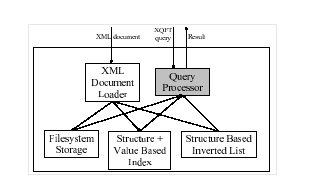
\includegraphics[width=0.5\textwidth]{img/quark_architecture.png}
  \caption{Quark architecture}
\end{figure}
Quark is an experimental full-text search engine capable of indexing and querying XML documents, and it uses the TexQuery query language (see below). Quark was developed as a research project at Cornell University by Jayavel Shanmugasundaram and his associates.
\begin{figure}[!h]
  \centering
    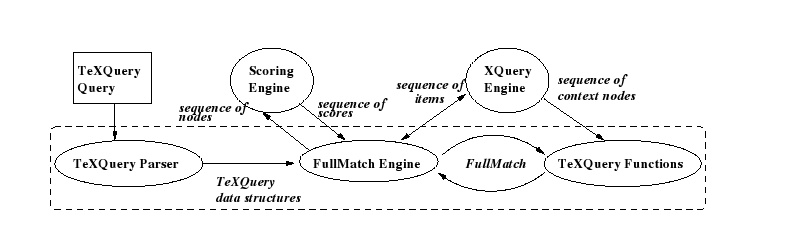
\includegraphics[width=1\textwidth]{img/texquery_architecture.png}
  \caption{TexQuery architecture}
\end{figure}
TexQuery is a query language extending upon Xquery with added full-text search capabilities. These extensions do not necessarily conform to the W3C recommendation, however TexQuery is an early precursor to the current W3C recommendation \cite{TEXQ00}, in whose development Shanmugasundaram actively participates.

\subsubsection{Galatex}
\begin{figure}[!h]
  \centering
    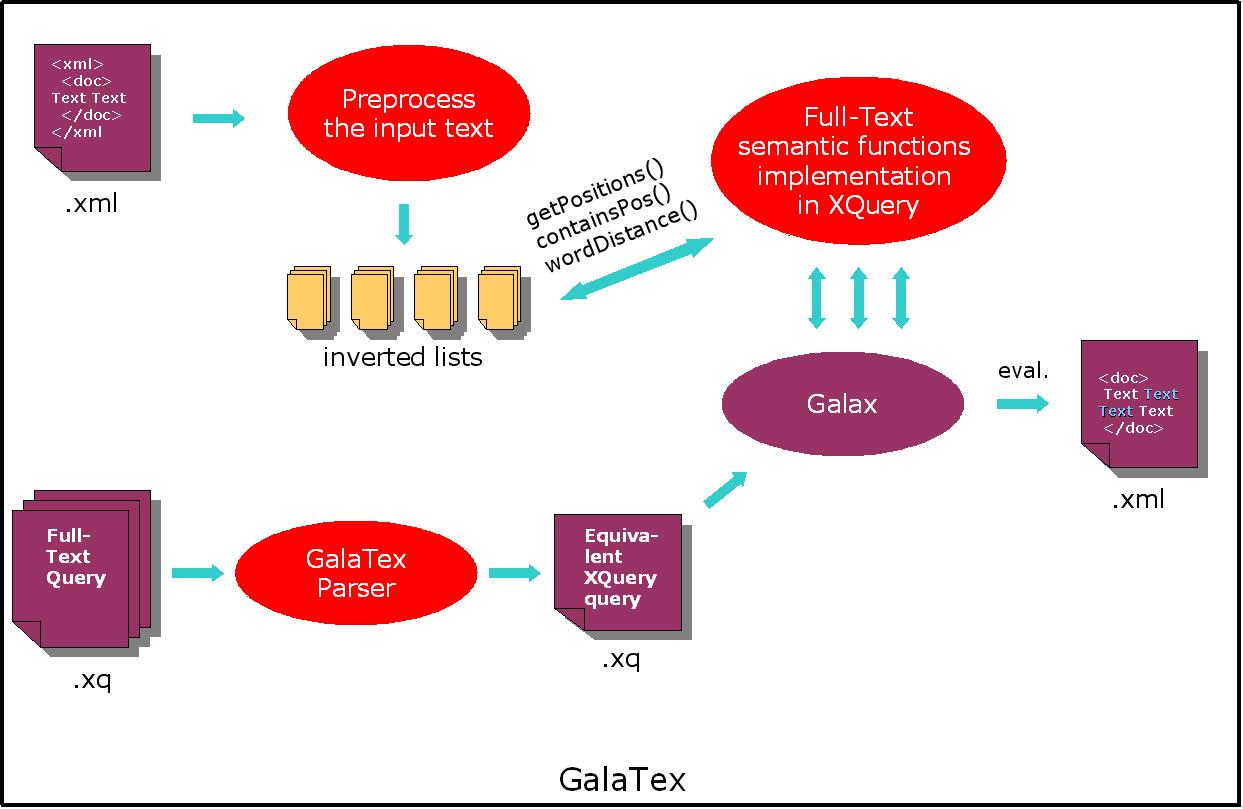
\includegraphics[width=1\textwidth]{img/galatex_architecture.png}
  \caption{Galatex architecture}
\end{figure}
GalaTex is a complete implementation of the Xquery 1.0 and Xpath 2.0
specifications with full-text extensions. GalaTex is an extension of Galax,
which is a generic Xquery engine. The XQFT query is parsed and converted to an
equivalent Xquery query which is passed to the Galax query engine. The GalaTex
source code is licensed under a non-commercial license developed to AT\&{}T 
\footnote{http://www.galaxquery.com/galatex/LICENSE} and is available at the
GalaTex website \cite{galatex}.

\subsubsection{Pathfinder}
\begin{figure}[!h]
  \centering
    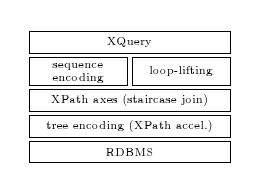
\includegraphics[width=0.5\textwidth]{img/pathfinder_architecture.png}
  \caption{Pathfinder architecture / development stack}
\end{figure}
The Pathfinder project is an XQuery parser running on top of relational database systems, namely MonetDB. The goal of the Pathfinder project is to investigate how relational database technology can be utilized to create a scalable and efficient XQuery implementation. However, the Pathfinder project has, at the current time of writing, no support for full text extensions. A future version of Pathfinder is planned to be capable of emitting SQL code generated from the XQuery parse tree. This illustrates the Pathfinder systems capabilities of interoperating with relational database systems.

Pathfinder is written in C, and the XQuery parser is a generated using standard Flex and Bison compiler generator tools.

\subsubsection{SaXon}
SaXon is an open source XSLT and XQuery processor. It is being actively developed by Michael Kay, and is licensed under the Mozilla Public License (MPL). SaXon conforms to the XSLT 2.0, XQuery 1.0 and XPath 2.0 recommendations by the W3C as of 23rd of january, 2007.

\subsubsection{Natix}
\begin{figure}[!h]
  \centering
    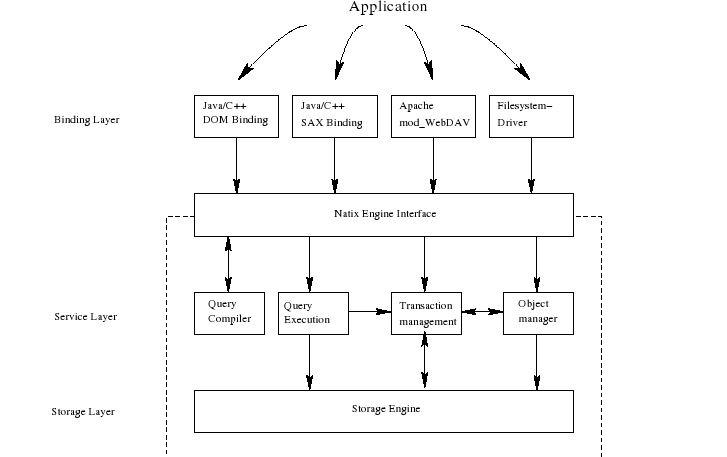
\includegraphics[width=1\textwidth]{img/natix_architecture.png}
  \caption{Natix architecture}
\end{figure}
Natix is an XML database system for persistent storage of XML, and provides access through DOM and SAX interfaces, as well as the option of performing XPath queries.
%Relasjonsalgebra
\section{Relational Algebra}
\label{sect:theory:relAlg}

The relational model for database management was introduced for the first time by Edgar Frank Coddin
1974\cite{TDT4225}. It was based on relational algebra which is an offshoot of first-order logic. Several terms
are used when talking about relational algebra \cite{gordonRussel}\cite{newYorkDB}\cite{sudarshan}:
\begin{itemize}
\item \textbf{Set}: A mathematical definition for a collection of objects which contains no duplicates
\item \textbf{Domain}: A \textit{set} of atomic values
\item \textbf{Attribute}: A real world role played by a named \textit{domain}
\item \textbf{Tuple}: A collection of \textit{attributes} which describe some real world entity
\item \textbf{Relation}: A \textit{set} of \textit{tuples}
\item \textbf{Degree}: The number of \textit{attributes} of a \textit{relation}. Sometimes called arity.
\item \textbf{Cardinality}: The number of \textit{tuples} in a \textit{relation}
\item \textbf{Union compatible}: Two relations $R$ and $S$ are union compatible if and only if they have the same
	\textit{degree} and the \textit{domains} of the corresponding \textit{attributes} are the same.
\end{itemize}

It should be noted that often relational algebra is based on ``bag'' semantics rather than set semantics. A
``bag'' may contain duplicates unlike sets. Removal of duplicates can be a very costly operation in terms of
computer resources.

\subsection{Primary Operators}
\label{sect:theory:relAlg:primOper}
The primary operators is a set of operators which constitutes the base of an algebra. Other operators can be
defined in terms of the primary ones. If one of the primary operators is excluded, the algebra will loose some of
it's expressiveness. The primitive operators of Codd's algebra are: selection, projection, union, difference,
cross product and rename (later added for the sake of the named relational algebra).

\subsubsection{Selection}
\label{sect:theory:relAlg:selection}
Selection is a unary operator, and is used to obtain a subset of the tuples of a relation that satisfy a select
condition. The resulting relation may have fewer tuples but it will have the same degree as the original relation.
It is sometimes called restriction to avoid confusion with SELECT in SQL. The
operator is often symbolised by \emph{s}igma:
\begin{equation*}
\sigma_{C}(R)
\end{equation*}
Where $R$ is a relation and $C$ is the select condition: a truth value or an expression yielding a truth value.
The expression can be made up of any combination of the logical operators \begin{math}\{ \wedge, \vee,
\neg\}\end{math}. Figure \ref{fig:theory:select} shows an example of a select operation.

\begin{figure}[h]
\centering
\begin{tabular}{lcr}
		\begin{tabular}{|c|c|} \hline
			\multicolumn{2}{|c|}{\textbf{R}} \\ \hline
			\textbf{Letter} & \textbf{Number} \\ \hline
			A & 1 \\ \hline
			A & 3 \\ \hline
			A & 6 \\ \hline
			B & 7 \\ \hline
		\end{tabular}  &
		\begin{math} \sigma _{Letter='A' \wedge Number > 2}(R) = \end{math}
		\begin{tabular}{|c|c|} \hline
			\multicolumn{2}{|c|}{} \\ \hline
			\textbf{Letter} & \textbf{Number} \\ \hline
			A & 3 \\ \hline
			A & 6 \\ \hline
		\end{tabular} 

\end{tabular}
\caption{Example showing the selection operator}
\label{fig:theory:select}
\end{figure}

\subsubsection{Projection}
\label{sect:theory:relAlg:projection}
Projection is also a unary operator, and is used to obtain a subset of the attributes of a relation. The resulting
relation will have an equal or lower degree than the original relation. In the case of duplicates being produced
as a result of omitting some attributes, the resulting relation will have fewer tuples than the original.
\emph{P}i is often used to symbolise the operation:
\begin{equation*}
\pi _{attr}(R)
\end{equation*}
Where $R$ is a relation and $attr$ is the set of attributes to be returned from $R$. Figure
\ref{fig:theory:project} shows an example of a projection. \begin{figure}[h]
\centering
\begin{tabular}{lcr}
	\begin{tabular}{|c|c|c|} \hline
	\multicolumn{3}{|c|}{\textbf{R}} \\ \hline
	\textbf{Let} & \textbf{Num} & \textbf{Sym} \\ \hline
	A & 1 & \% \\ \hline
	B & 1 & \% \\ \hline
	C & 3 & \# \\ \hline
	\end{tabular} &
	\begin{math} \pi _{Num, Sym} (R) = \end{math}
	\begin{tabular}{|c|c|} \hline
	\multicolumn{2}{|c|}{} \\ \hline
	\textbf{Num} & \textbf{Sym} \\ \hline
	1 & \% \\ \hline
	3 & \# \\ \hline
	\end{tabular}
\end{tabular}	
\caption{Exaple showing the projection operator}
\label{fig:theory:project}
\end{figure}

\subsubsection{Union and Difference}
\label{sect:theory:relAlg:unionAndDiff}
Union and difference are two binary operators analogous with union and difference operators in set theory. The
relational algebra version of the operators requires that the relations involved are union compatible.

The union of two relations returns a relation which includes all the tuples that are in either or both of the
original relations. As the result is also a relation, any potential duplicates will be removed. The operation is
commutative, and the returned relation will have the same degree as the two relations involved. A union between
two relations are often symbolised thus:
\begin{equation*}
R \cup S
\end{equation*}
Where $R$ and $S$ are relations.

The difference of two relations R and S is a relation that contains all the tuples that are in R but not in S. The
returned relation will, as was the case with union, have the same degree as the two relations involved. A
difference between relations $R$ and $S$ is written like this:
\begin{equation*}
R - S 
\end{equation*}

\subsubsection{Cross Product}
\label{sect:theory:relAlg:crossProduct}
The cross product operator is sometimes referred to as the cartesian product operator. As with union and
difference, this operator also stems from set theory. The operator is used to combine all tuples in one relation
with all the tuples from another. The returned relation will have a degree equal the sum of the degrees of each of
the original relations, and a cardinality equal the product of the cardinalities. The operator is commutative and
written as a cross:
\begin{equation*}
R \times S = S \times R
\end{equation*}
Where $R$ and $S$ are relations. Figure \ref{fig:theory:crossproduct} shows an
example of a cross product. \begin{figure}[h]
\begin{tabular}{ccccc}
	\begin{tabular}{|c|} \hline
	\textbf{R} \\ \hline
	\textbf{Let} \\ \hline
	A \\ \hline
	B \\ \hline
	\end{tabular}
	&
	\begin{math} \times \end{math}
	&
	\begin{tabular}{|c|c|} \hline
	\multicolumn{2}{|c|}{\textbf{S}} \\ \hline
	\textbf{Num} & \textbf{Let} \\ \hline
	1 & C \\ \hline
	2 & A \\ \hline
	\end{tabular}
	&
	\begin{math} = \end{math}
	&
	\begin{tabular}{|c|c|c|} \hline
	\multicolumn{3}{|c|}{} \\ \hline
	\textbf{R.Let} & \textbf{S.Num} & \textbf{S.Let} \\ \hline
	A & 1 & C \\ \hline
	A & 2 & C \\ \hline
	B & 1 & A \\ \hline
	B & 2 & A \\ \hline
	\end{tabular}
\end{tabular}
\centering
\caption{An example of cross product.}
\label{fig:theory:crossproduct}
\end{figure}

\subsubsection{Rename}
\label{sect:theory:relAlg:rename}
Rename is a unary operator used to rename a relation and/or a subset of its attributes. The resulting relation
will be equal to the original one in all aspects except maybe some of its name properties. The Greek letter
\emph{r}ho is often used to mark the presence of the rename operator:
\begin{equation*}
\rho _{S}(R)
\end{equation*}
Where $R$ is the relation being renamed, and $S$ is a relational scheme. $S$ is on the form $T _{(a _{1},...a
_{n})}$ for a n-degree relation, where $T$ is the new relation name and $a _{1},...a _{n}$ is the new names for
relation $R$'s attributes from $1$ to $n$. The degree of the scheme must be the same as the degree of the relation
being operated on.

\subsection{Derived Operators}
\label{sect:theory:relAlg:derivedOper}
None of the six primary operators can be expressed as a combination of any of the others. In contrast, some useful
operators can be derived using one or more of the primary ones. Most notably among these are intersection and join.

\subsubsection{Intersection}
\label{sect:theory:relAlg:intersection}
Intersection is the fourth mentioned operator that stems from set theory. It is a binary operator, and the
resulting relation will contain the set of tuples that are in both of the relations operated on. It can be
expressed with the help of the difference operator, and hence require that the input relations are union compatible:
\begin{equation*}
R \cap S = R-(R-S)
\end{equation*}

\subsubsection{Joins}
\label{sect:theory:relAlg:joins}
Joins are a group of operators that all are derived from the primary operators with the cross product as a base.
Among the operators in this group is natural join, theta-join, equi-join, anti-join, semi-join, outer joins and
division. Some of these will be presented in this section.

\paragraph{Natural Join.}
\label{sect:theory:relAlg:naturalJoin}
Natural join is a binary operator that returns a relation consisting of all combinations of tuples in input
relations that are equal on their common attribute names. The result relation will have a degree equal to the sum
of the degrees of the two original relations subtracted the number of common attributes. Natural join can be
expressed as a combination of cross product, projection and selection:

\begin{equation*}
R \bowtie S = \pi_{a_{1},..., a_{n},R.b_{1},...,R.b_{n},c_{1},...,c_{n}}( \sigma _{R.b_{1}=S.b_{1} \wedge ... \wedge R.b_{n}=S.b_{n}}(R \times S))
\end{equation*}

Where $R$ and $S$ are relations, $b_{1},..,b_{n}$ are the common attributes, $a_{1},..,a_{m}$ are the attributes
unique to $R$ and $c_{1},...,c_{k}$ are the attributes unique to $S$. A rename operator can lastly be used to
remove the prefix of the common attributes.

\paragraph{Equi-join and Theta-join.}
\label{sect:theory:relAlg:equiAndThetaJoin}
Theta-join returns a relation which is a combination of all the tuples in the two input relations that satisfy a
condition $C$. $C$ is in the form $a \theta b$, where $a$ is a attribute name from one relation, $b$ is an
attribute from the other and $ \theta $ is a binary operator in the set $ \{ <, \leq , =, \geq , >  \} $. An
equi-join is a theta-join where the binary operator in the condition is the equality operator. Theta-join can be
expressed as a combination of selection and a cross product:

\begin{equation*}
R \bowtie _{a \theta b}S = \sigma _{a \theta b}(R \times S)
\end{equation*}

\paragraph{Division.}
\label{sect:theory:relAlg:division}
Division in relational algebra can be described as the inverse operator of cross product, in the same way division
and multiplication are inverse in natural numbers calculus -- i.e. they are not inverse if the division gives a
residue:

\begin{equation*}
(R \times S) \div R = S ~~and~~ (R \times S) \div S = R
\end{equation*}

The resulting relation after a division contains the attribute values of the divisor relation that are associated
with every member of the dividend relation\cite{makeDiv}. The operation may be better explained as a
combination of cross product, projection and difference:

\begin{equation*}
R \div S = \pi _{a_{1},...,a_{n}}(R) - \pi _{a_{1},...,a_{n}}((\pi _{a_{1},...,a_{n}}(R) \times S) - R)
\end{equation*}

Where $R$ and $S$ are relations and $a_{1},...,a_{n}$ are the attributes unique to $R$.

\paragraph{Semi-join.}
\label{sect:theory:relAlg:semiJoin}
Semi-join is a binary operation which returns a relation with the attributes of the first relation, and all the
tuples in this same relation for which there is a tuple in the second relation that is equal on their common
attributes. Semi-join can be described with the project and natural-join operators:

\begin{equation*}
R \ltimes S = \pi _{a_{1},...,a_{n}}(R \bowtie S)
\end{equation*}

Where $R$ and $S$ are relations, and $a_{1},...,a_{n}$ are the attributes unique to $R$.

\paragraph{Anti-join.}
\label{sect:theory:relAlg:antiJoin}
The anti-join operator is very similar to the semi-join operator (and is also sometimes referred to as the
anti-semi-join), except that it returns all the tuples in the first relation for which there is no tuple in the
other relation on their common attributes. It can be described with help of semi-join and difference:

\begin{equation*}
R \rhd S = R - R \ltimes S
\end{equation*}

Where $R$ and $S$ are relations.

\paragraph{Outer Joins.}
\label{sect:theory:relAlg:outerJoin}
The outer joins is in many ways as the natural join, except the resulting relation will include some extra
tuples based on one or both of the input relations. The right outer join $(\times=)$ will return a relation with
all the tuples from a natural join between the first (left) and the second (right) relation, as well as the tuples
from the right relation that did not match any tuples from the left one on their common attributes. These extra
tuples will have the value NULL in the result relation for all attributes that were unique to the left relation.
The left outer join $(=\times)$ is analogous with the right version, the only difference is that the extra tuples
will be based on the left input relation. The result relation of a full outer join $(=\times=)$ will have extra
tuples based the ones that did not find a match in both input relations.

\section{Parsing and syntax trees}
\label{sect:parser_and_syntaxtrees}
The act of parsing is the process of analyzing a series of tokens and construct
a grammatical structure (syntax tree) based on a formally specified grammar. In
figure \ref{figure:parser:overview}, the parser component of a generic
compiler/interpreter is shown. 

\begin{figure}[h]
  \centering
    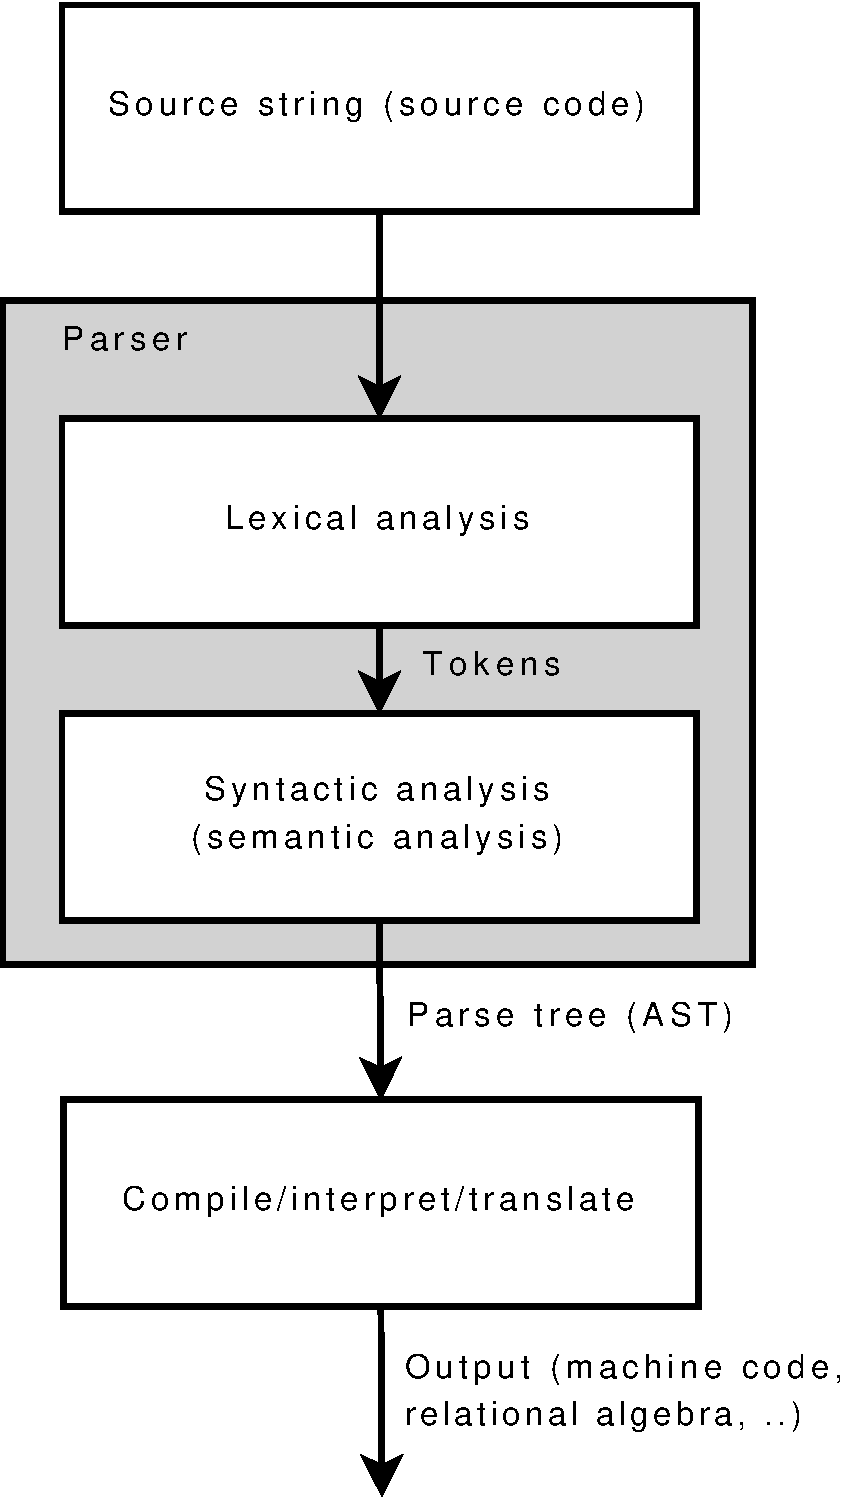
\includegraphics[scale=0.40]{diagrams/parser_overview}
  \caption{Typical compiler/interpreter data flow}
  \label{figure:parser:overview}
\end{figure}

\subsection{Common parser technologies}
There are two common types of parser technologies, \textit{top-down} and
\textit{bottom-up} parsers. As their names imply, these technologies differ in
the sense that top-down parsers will attempt to match production rules to the
input top-down, while bottom-up parsers will start at the ``bottom'' on the
terminal symbols and combine them into production rules. Often this is
implemented as a process of shift and reduce operations using stacks to hold
production rules and terminal symbols.

We refer to \cite{compiler_tech} for further in-depth information about parser
technologies, however it is important to note that typically a top-down parser
based on an LL\footnote{LL is a Left-to-right, Leftmost derivation
parser, using a top-down approach}-grammar with low token lookahead (typically
one token lookahead, aka LL(1)) will perform better and be subject to a high
number of well-defined optimizations, out of which a few are described in
\cite{compiler_tech} and \cite{DBLP:books/cu/Appel1998c}.

\subsection{Parser generators}
For large grammars, writing a parser by hand from the ground up may turn out to
be a substantial amount of work. To eliminate this, a large number of
\textit{parser generators} exist. Most of these parser generators have a very
similar set of functionality. From a formal grammar, often in a notation
similar to BNF, the parser generator will output the source code for a
complete parser for the given grammar. Ideally, the maintainability of this
generated parser could be reduced to simply changing the grammar specification,
without actually modifying the generated source code.

\begin{figure}[h]
  \centering
    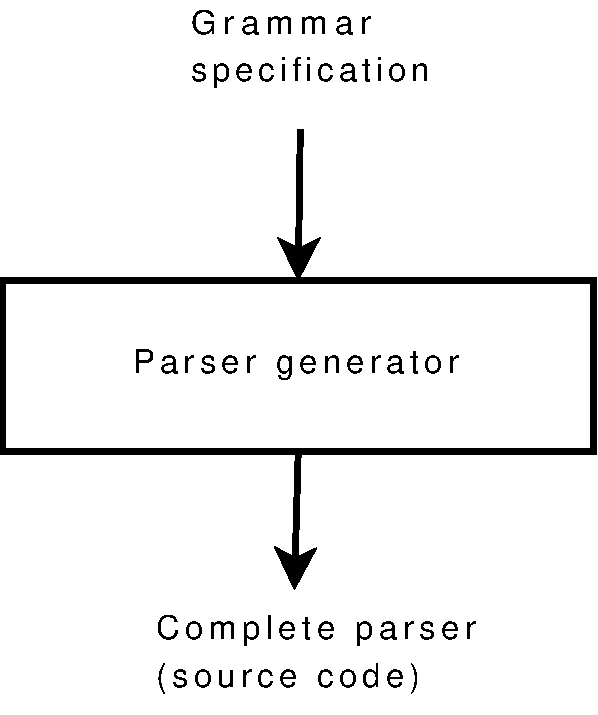
\includegraphics[scale=0.40]{diagrams/parser_generator}
  \caption{Automatic parser generation workflow}
  \label{figure:parser:generator}
\end{figure}

Several parser generators exists, covering several target languages and
overlapping in terms of functionality and features. As expected, the most
common parser generators will generate either top-down or bottom-up parsers
(described earlier in this section). Typical examples of bottom-up parser
generators are yacc (and derivatives), CUP, GOLD, and SableCC. Some popular
top-down parsers include JavaCC, ANTLR, Spirit, and Coco/R.

A comparison of some of the most popular parser generators were made in
\cite{ourselves} for the development of the XQFT Parser (see next subsection 
\ref{sect:theory:xqftparser}), and out of these the ANTLR parser generator was
chosen. We will not reiterate the features of ANTLR in this document, however
it is important to note that ANTLR generates predicated LL(*)-parsers based on
LL-compliant grammars. This choice was made due to the XQuery BNF specification
which is claimed to be LL(1) (one token lookahead).

\subsection{The XQFT Parser project}
\label{sect:theory:xqftparser}
The XQFT Parser\cite{ourselves} was developed as a part of an academic project
at the Department of Computer and Information Science (IDI) at the Norwegian
University of Science and Technology (NTNU) throughout the autumn of 2007.

In this project the ANTLR parser generator was utilized to generate a
LL(*)-parser based on the W3C specification\cite{w3c01} for XQuery with
full-text extensions.

The output from this parser are carefully crafted abstract syntax trees which
are well suited for translation into other representations.

\subsubsection{AST construction}
The abstract syntax tree is constructed by specifying tree rewrite rules in the
grammar file (the tree rewrite rules were extensively covered in \cite{ourselves}, section
4.5). The tree consists of nodes instantiated from the
\verb!no.ntnu.xqft.parse.XQFTTree! class. To compensate for missing tokens to
determine tree context, the XQFT Parser employs the use of imaginary tokens.
These are simply tokens that do not exist in the input stream, they only have
an associated name and no specific token. These imaginary tokens are typically
used where there are no ``real'' tokens available to represent the proper
semantic or contextual meaning.

One example can be seen in figure \ref{figure:parser:imaginary_tokens_path},
where the imaginary tokens AST_MODULE, AST_PATHEXPR_SGL, and AST_STEPEXPR have
been injected into the tree.

\begin{figure}[h]
  \centering
    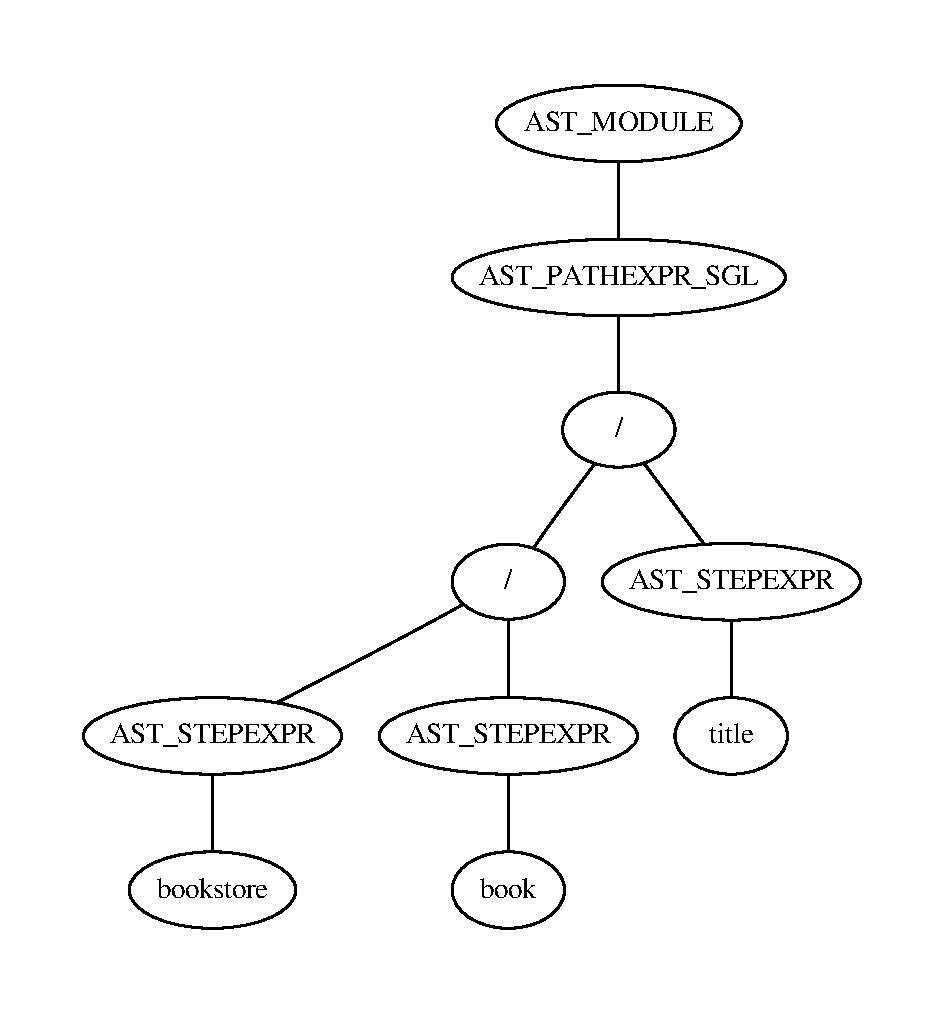
\includegraphics[scale=0.50]{diagrams/path1}
  \caption{Example of injected imaginary tokens}
  \label{figure:parser:imaginary_tokens_path}
\end{figure}

The details of injection of imaginary tokens is explained in detail in
\ref{ourselves}, section 

\subsection{Tree parsing}
Tree parsing, henvise til metode eller flytte greiene fra metode og hit? Eller
noe.

\begin{itemize}
  \item Kort om forskjellige parser-teknologier
  \item Hvordan parseren vaar fungerer
  \item Hvordan ASTen ser ut\ldots kanskje nesten en egen subsection til
  dette.. iallefall i generelle trekk? hmmmmmz
  \item Syntax-tr\ae r og tre-parsing
  \item AST\_PATHEXPR\_SGL holder enkeltslash i begynnelsen av pathExprz
  \item Imagin\ae re tokens, og evt snakke om hvilke vi har lagt til i
  implementation?
\end{itemize}

\section{Loop Lifting}
\label{sect:trans:loop_lifting}
\label{sect:theory:loop_lifting}
Loop lifting is a method of translating XQuery iteration expressions into relational algebra. The method was
developed by Torsten Grust and Jens Teubner and originally presented in \cite{pathfinder_mothertongue}. It is a
part of the Pathfinder project\cite{pathfinderHome} (see section \ref{sect:theory:pathfinder}).

In this section we will present Loop Lifting mainly based on the two articles \cite{pathfinder_purelyRelational}
and \cite{pathfinder_mothertongue}. The articles present the method for a subset of XQuery Core (Pathfinder
rewrites queries to Core, see section \ref{sect:theory:pathfinder}), of which we will only present the elements
relevant in a comparison between Loop Lifting and the Tainting Dependencies method. Thus, the translation of path
expressions and XML-element construction will not be handled, as pathfinder's XML-tree representation(section
\ref{sect:theory:pathfinder}) is incompatible with MARS.

Pathfinder generates relational operator directed asyclic graphs (DAGs) rather than operator trees. The Loop
Lifting method does not require such a structure, but as we will see, it will gain advantage by it, as much
evaluation relies on earlier evaluations. 

Accompanying the translation method is also methods for analysis, simplification and optimisation of the generated
relational algebra, such as the Peep-Hole plan simplification\cite{pathfinder_purelyRelational}.


\subsection{Operators}
\label{sect:trans:ll:Operators}
Loop-lifting utilises a set of relational algebra operators, out of which the ones used in this chapter is
presented in table \ref{tab:trans:ll:Operators}.
\begin{table}[h]
\centering
\begin{tabular}{l|l} 
$\pi_{a_{1}:b_{1},\ldots,a_{n}:b_{n}}$ 	& projection and renaming	\\ 	\hline
$\sigma_{a}$					   		& selection             	\\ 	\hline
$\dot\cup$ 							& disjoint union			\\	\hline
$\times$								& cartesian product			\\	\hline
$\bowtie_{a=b}$							& equi-join					\\ 	\hline
$\varrho_{b:(a_{1},\ldots,a_{n})/p}$	& numbering operator		\\	\hline
$\circledcirc_{b:(a_{1},\ldots,a_{n})}$	& $n$-ary arithmetic/comparison operator $\circ$ \\ \hline
\scriptsize \begin{tabular}{c|c} $a$& $b$\\\hline\end{tabular} & literal table
\end{tabular}
\caption[of the Pathfinder relational algebra]{Operators of the Pathfinder relational algebra. $a$, $b$ and $p$
represents attributes}
\label{tab:trans:ll:Operators}
\end{table}

Most of the operators are quite standard, and can easily be understood by comparing with the operators from
general relational algebra (section \ref{sect:theory:relAlg}) and MQL (section \ref{sect:method:marsOperators}).

Only a very restricted selection
is utilised, written $\sigma_{a}$, which only returns tuples satisfying $a \neq 0$.  Considering the numbering
operator, $p$ denotes the partitioning attribute, $(a_{1},\ldots,a_{n}$ the attributes to be sorted on and $b$ is
an added attribute holding the result of the
numbering (equal to the proposed \textsf{numberate}-operator of MQL, section \ref{sect:method:marsAddedOperators}).
{\scriptsize{\begin{tabular}{c|c}$a$&$b$\\\hline\end{tabular}}} represents the creation of a relation with
attributes $a$ and $b$.

Operator $\circledcirc_{b:(a_{1},\ldots,a_{n})}$ will evaluate the arithmetic/comparison expression $a_{1} \circ
\ldots \circ a_{n}$ and place the result in $b$. Where $\circ \in \left\{ +,- , <, =, \ldots  \right\} $.


\subsection{Basics}
\label{sect:trans:ll:Basics}
XQuery expressions evaluate to finite, ordered sequences of items. As a sequences are one-dimensional, it can be
represented by a single relation where each tuple encodes a sequence item. The order of the sequence is
maintained by an attribute \textit{pos}. The value of the item is held in an attribute \textit{item}. 

During this section concerning Loop Lifing, variables, expressions and scopes is denoted like this (ref. section
\ref{sect:theory:xquery:Flwor}):
\[
s \left\{
\begin{array}{l}
\qquad \qquad \quad \vdots \\
\mbox{\texttt{for \$}}v_{0}\mbox{\texttt{ in }} e_{0} \mbox{\texttt{ return}} \\
\quad s_{0} \left\{ e_{0}' \right. \\
\qquad \qquad \quad \vdots
\end{array}
\right.
\]

Generally, a scope $s_{x \cdot y}$ identifies the $y$th child scope of scope $x$, $x \in \left\{
\mathbb{N}\right\}, y \in \left\{ \mathbb{N} \right\}$. Expression $e_{x\cdot y}$ evaluates to an iterator sequence
and is bound to the variable $v_{x \cdot y}$. $e_{x \cdot y}'$ constitutes the coresponding iterator body, and $I_{x \cdot y}$ the whole iterator expression.

$q_{x}(e)$ is used to denote the relational representation of expression $e$ in scope $s_{x}$.


\subsection{Constant Subexpressions}
\label{sect:trans:ll:ConstExprs}

For a iterator expression $i_{x}$ with $n$ iterations there exists a relation $loop_{x}$, consisting of a
single column, \textit{iter}, with values 1,2,\ldots,$n$. In the outermost scope, $loop$ has a single tuple with
the value 1.

A constant value $c$ in scope $s_{x}$ is \textit{lifted} like this:
\begin{equation}
q_{x}(c) =  loop_{x} \times \mbox{\scriptsize \begin{tabular}{c|c} \textit{pos}&\textit{item} \\
\hline 1 & \textit{c}
\end{tabular}}
\label{eq:ll:constLoopLift}
\end{equation}

A tuple ($iter,pos,item$) in a loop lifted relation for subexpression $e_{x}'$ can be understood as during the
$iter$th iteration, the item in position $pos$ in $e_{x}'$ has the value $item$.

\subsection{Bound Variables}
\label{sect:trans:ll:boundVar}

An iterator sequence expression $e_{x \cdot y}$ is evaulated in scope $s_{x}$. This sequence is then iterated over
and each item is successively bound to the iterator variable $v_{x \cdot y}$. The evaluation of $e_{x \cdot y}'$
is in scope $s_{x \cdot y}$ and may utilise these bindings. 

Considering this, a representation of $v_{x \cdot y}$ in scope $s_{x \cdot y}$ may therefore be calculated by
retaining the values of $q_{x}(e_{x \cdot y})$, introducing a $iter$ attribute with consecutive numbers and
holding the $pos$ attribute to the constant value 1. In terms of algebra, the representation of $v_{x \cdot y}$ is
computed like this:
\begin{equation}
q_{x \cdot y}(\mbox{\texttt{\$}}v_{x \cdot y}) = \mbox{\scriptsize \begin{tabular}{c} $pos$ \\\hline 1
\end{tabular}} \times \pi_{iter:inner,item}(\varrho_{inner:(iter,pos)}(q_{x}(e_{x \cdot y})))
\label{eq:ll:qxy_vxy}
\end{equation}
The introduction of the $inner$ attribute is used to denote evaluation of the loop in scope $s_{x \cdot y}$. The
$iter$ attribute of $q_{x}(e_{x \cdot y})$ can be viewed as an atttribute $outer$, as it denotes the iterations in
the outer loop of scope $s_{x}$.

Loop lifting requires maintenance of a $loop$ relation to ensure independent iterations. The iterator body in
scope $s_{x \cdot y}$ needs to be evaluated once for each binding of the iterator variable $v_{x \cdot y}$.
Thus, the $loop$ relation needs to be redifined based on $q_{x \cdot y}(v_{x \cdot y})$:
\begin{equation}
loop_{x \cdot y} = \pi_{iter}(q_{x \cdot y}(v_{x \cdot y}))
\label{eq:ll:loopxy}
\end{equation}


\subsection{Free Variables}
\label{sect:trans:ll:freeVar}

XQuery expressions may use any iterator variable bound in enclosing scopes. That is, $v_{x}$ bound in
scope $s_{x}$ may also be referred to within any of its child scopes. When looking at one of these child scopes,
$s_{x \cdot y}$, by itself, the variable $v_{x \cdot y}$ appears to be a free variable.

Consider a iterator expresion $I_{x \cdot y}$ within another iterator expression $I_{x}$, both with iterator
sequences of length two. If $v_{x}$ is referred to within scope $s_{x \cdot y}$, from $s_{x \cdot y}$'s point of
view, $v_{x}$ is free. For each binding of $v_{x}$ in the \textit{outer} iteration expression, two
evaluations of the \textit{inner} iteration expresion occur. A relation capturing the relationship between number
of iterations of these two iterator expressions can be defined like this:

\begin{center}
\begin{tabular}{|c|c|}\hline
\textit{outer}	& \textit{inner} 	\\ \hline
1				& 1		\\ \hline
1				& 2		\\ \hline
2				& 3		\\ \hline
2				& 4		\\ \hline
\end{tabular}
\end{center}

Where a tuple $(outer, inner)$ is read as for the $inner$th iteration of the inner iterator expression, the outer
iterator expression is in its $outer$th iteration. This relation is called $map_{x, x\cdot y}$ as it maps
representations between scopes $s_{x}$ and $s_{x \cdot y}$. It can be calculated like this:
\begin{equation}
map_{x, x\cdot y} = \pi_{outer:iter,inner}(\varrho_{inner:(iter,pos)}(q_{x}(e_{x \cdot y})))
\label{eq:ll:mapx_xy}
\end{equation}

With this relationship defined it is now possible to represent the free variable $v_{x}$ in the scope $s_{x \cdot
y}$ with the help of an equi-join:
\begin{equation}
q_{x \cdot y}(\mbox{\texttt{\$}}v_{x}) = \pi_{iter:inner, pos,
item}(q_{x}\left(\mbox{\texttt{\$}}v_{x})\bowtie_{iter=outer} map_{x, x \cdot y}\right)
\label{eq:ll:qxy_vx}
\end{equation}

\subsection{Mapping Back}
\label{sect:trans:ll:mappingBack}

All steps and equations this far have been helpful to represent sequences and variables in a lower scope level. But
the result of a query will have to be in form of its representation in the outermost scope $s$. So a way to
represent an expression $e_{x,y}'$ in its scope's parent scope $s_{x}$ is needed. Once again the $map$ relation
may be of use, combined with an equi-join:
\begin{equation}
q_{x}(e_{x \cdot y}') =
\begin{array}{l}
 \pi_{iter:outer, pos:pos1, item}(\\ \qquad\varrho_{pos1:(iter,pos)/outer}(q_{x \cdot
y}(e_{x \cdot y}')\bowtie_{iter = inner}map_{x, x \cdot y}))
\end{array}
\label{eq:ll:qx_exymark}
\end{equation}


\subsection{Other Expression Types}
\label{sect:trans:ll:OtherExpr}

The sequence construction $e_{1}$\texttt{, }$e_{2}$ is essentially a disjont union of the
relational representations of the expressions, that is, $q_{x}(e_{1})$ and $q_{x}(e_{2})$. By temporarily adding a
attribute $ord$ to these relations before a renumbering of the result with $\varrho$, the proper ordering of the
sequence is aquired. Construction of sequences can therefore be expressed like this:
\begin{equation}
q_{x}(e_{1}\mbox{\texttt{, }}e_{2})=
\begin{array}{l}


\pi_{iter,pos:pos1,item}
\left( \right.\\ \qquad

\varrho_{pos1:(ord,pos)/iter}
	\left( \right. \\ \qquad \qquad
	\left. \left.
		\left(
		\frac{ord}{1} \times q_{x}(e_{1})
		\right)
		\dot\cup
		\left(
		\frac{ord}{1} \times q_{x}(e_{2})
		\right)		
	\right)
\right)
\end{array}
\label{eq:ll:secuence}
\end{equation}

The $\circledcirc$ operator meets the requirement of evaluating comparison and arithmetic operations on atomic
values. Given two XQuery values $e_{1}$ and $e_{2}$ in multiple iterations, with relational representations as before,
the expression $e_{1}$ \texttt{ + } $e_{2}$ can be translated by first joining $q_{x}(e_{1})$ and $q_{x}(e_{2})$
on their iteration number, i.e. $iter$. Then, for each tuple, store the sum of the values of both of the $item$
attributes, before cleaning up the resulting relation with a project. Expressed as an equation, the translation of
sum expressions looks like this:
\begin{equation}
q_{x}(e_{1} \mbox{\texttt{ + }} e_{2}) =
\begin{array}{l}
\pi_{iter,pos,item:res}\left(\right. \\ \qquad
\oplus_{res:(item,item')}
\left( \right. \\ \qquad \qquad

	q_{x}(e_{1})
	\bowtie_{iter = iter'}
	 \\ \qquad \qquad \qquad
	\left.\left(\pi_{iter':iter, item':item}(q_{x}(e_{2}))
	\right)
\right)
\end{array}
\label{eq:ll:sumexpr}
\end{equation}

The \texttt{if(}$e_1$\texttt{) then }$e_2$\texttt{ else }$e_3$, is one of the more complex translations of loop
lifting. First the boolean expression $e_1$ is compilated. The result is split into two new loop relations,
$loop1$ and $loop2$, which uses selection on all $true$ and $false$ values respectively. $loop2$ is used as current
$loop$ relation for the compilation of $e_2$ and $loop3$ as $loop$ relation for the mapping of $e_3$. A equi-join with
their corresponding $loop$ relation on $iter$ will filter out all unnnecesary iterations. The result is the union
of both branches.

\begin{equation}
\begin{array}{l}
q_{x}(\mbox{\texttt{if }}e_1\mbox{\texttt{ then }}e_2\mbox{\texttt{ else }}e_3) = \\ \qquad
\begin{array}{l}
\pi_{iter,pos,item}(q_{x}(e_2)\bowtie_{iter=iter'}(\pi_iter':iter(loop2))\,\dot\cup \\ \qquad
\pi_{iter,pos,item}(q_{x}(e_3)\bowtie_{iter=iter'}(\pi_iter':iter(loop3)) \\
loop2 = \pi_{iter}(\sigma_{item=TRUE}(q_{x}(e_1))) \\
loop3 = \pi_{iter}(\sigma_{item=FALSE}(q_{x}(e_1))) \\
\end{array}
\end{array}
\label{eq:ll:ifthenelse}
\end{equation}

\subsection{Example}
\label{sect:trans:ll:example}

Only looking at equations may be a bit too abstact to fully understand Loop Lifting. To concretise we will present
a simple example of evaluating a query with the method and show intermediate results. The naming of expressions,
scopes and variables will, where possible, be the same as earlier in this section. This query is the basis of this
evaluation:

\begin{figure*}[h!]
\centering
\begin{math}
s\left\{
\begin{array}{l}
\mbox{\texttt{for \$v0 in (10,20) return}} \\ \;
s_{0}\left\{
\begin{array}{l}
\mbox{\texttt{(\$v0, for \$v00 in (7,8,9) return}} \\ \;
s_{0,0}\left\{ \mbox{\texttt{\$v0 + \$v00)}}\right.
\end{array}
\right.
\end{array}
\right.
\end{math}
\end{figure*}

The goal of the evaluation is, after all other calculations, to have a representation of $e_{0}'$ in scope $s$,
that is, $q(e_{0}')$. This is done by nesting inwards until the deepest scope, while calculating needed helping
relations on the way, before evaluating the subexpressions one by one as one nests outwards until the outermost
scope.

Firstly a representation of the outermost loop is needed. With the help of equation \ref{eq:ll:constLoopLift} we
find a representation of \texttt{(10, 20)} in scope $s$, $s(e_{0})$. Then, employing equation \ref{eq:ll:qxy_vxy}
yields \texttt{\$v0} in scope $s_{0}$, the result of which is shown in figure \ref{fig:trans:ll:q0_v0}.
$loop_{0}$ and $map_{\, ,0}$ can now be calculated by using equations \ref{eq:ll:loopxy} and \ref{eq:ll:mapx_xy}
and are shown in figure \ref{fig:trans:ll:loop0} and \ref{fig:trans:ll:map_0} respectevely (remember
$loop$ consists of a single tuple with value 1).

\begin{figure}[!h]
\centering
\subfigure[$q_{0}($\texttt{\$v0}$)$]{
%q0_v0
\begin{tabular}{|c|c|c|} \hline
$pos$	& $iter$	& $item$ \\ \hline
1		& 1			& 10 	\\ \hline
1		& 2			& 20 	\\ \hline
\end{tabular}
\label{fig:trans:ll:q0_v0}
%\caption{$q_{0}($ \texttt{\$v0} $)$}
}
\qquad \quad
\subfigure[$loop_{0}$]{

\begin{tabular}{|c|} \hline
$iter$ \\\hline
1 \\\hline
2 \\\hline
\end{tabular}
\label{fig:trans:ll:loop0}
%\caption{$loop_{0}$}
}
\qquad \quad
\subfigure[$map_{\, ,0}$]{
\begin{tabular}{|c|c|} \hline
$outer$ & $inner$ \\ \hline
1 & 1 \\ \hline
1 & 2 \\ \hline
\end{tabular}
\label{fig:trans:ll:map_0}
%\caption{$map_{\, ,0}$}
}
\label{fig:trans:ll:outerIntermediate}
\caption{Outer loop intermediate results}
\end{figure}

Before we evaluate the sequence expression in scope $s_0$, we need to evaluate the inner \texttt{for} loop. By the
same measure as with the outer loop we first calculate $q_{0\cdot 0}($\texttt{\$v00}$)$, $loop_{0 \cdot 0}$ and
$map_{0, 0 \cdot 0}$. The results are shown in figure \ref{fig:trans:ll:innerIntermediate}.

\begin{figure}[!h]
\centering
\subfigure[$q_{0\cdot 0}($\texttt{\$v00}$)$]{
\begin{tabular}{|c|c|c|} \hline
$pos$	& $iter$	& $item$ \\ \hline
1		& 1			& 7 	\\ \hline
1		& 2			& 8 	\\ \hline
1		& 3			& 9 	\\ \hline
1		& 4			& 7 	\\ \hline
1		& 5			& 8 	\\ \hline
1		& 6			& 9 	\\ \hline
\end{tabular}
\label{fig:trans:ll:q00_v00}
%\caption{$q_{0}($ \texttt{\$v0} $)$}
}
\qquad
\subfigure[$loop_{0 \cdot 0}$]{
\quad
\begin{tabular}{|c|} \hline
$iter$ \\\hline
1 \\\hline
2 \\\hline
3 \\\hline
4 \\\hline
5 \\\hline
6 \\\hline
\end{tabular}
\label{fig:trans:ll:loop00}
%\caption{$loop_{0}$}
\quad
}
\qquad 
\subfigure[$map_{0, 0 \cdot 0}$]{
\begin{tabular}{|c|c|} \hline
$outer$ & $inner$ \\ \hline
1 & 1 \\ \hline
1 & 2 \\ \hline
1 & 3 \\ \hline
2 & 4 \\ \hline
2 & 5 \\ \hline
2 & 6 \\ \hline
\end{tabular}
\label{fig:trans:ll:map0_00}
%\caption{$map_{\, ,0}$}
}
\caption{Inner loop intermediate results \label{fig:trans:ll:innerIntermediate}}
\end{figure}

To be able to calculate the sum-expression, $e_{0 \cdot 0}'$, we first need a representation of the variable
\texttt{\$v0} in scope $s_{0 \cdot 0}$. As this variable is a free variable in this scope, this is done by
applying equation \ref{eq:ll:qxy_vx} on $q_{0}($\texttt{\$v0}$)$ (figure \ref{fig:trans:ll:q0_v0}). This
result is shown in figure \ref{fig:trans:ll:q00_v0}. Now that we have both \texttt{\$v0} and \texttt{\$v00}
expressed in scope $s_{0 \cdot 0}$, we can employ equation \ref{eq:ll:sumexpr} to sum the two
variables together. The resulting relation can be seen in figure \ref{fig:trans:ll:q00_e00m}.

\begin{figure}[!h]
\centering
\subfigure[$q_{0\cdot 0}($\texttt{\$v0}$)$]{
\qquad 
\begin{tabular}{|c|c|c|} \hline
$pos$	& $iter$	& $item$ \\ \hline
1		& 1			& 10 	\\ \hline
1		& 2			& 10	\\ \hline
1		& 3			& 10	\\ \hline
1		& 4			& 20	\\ \hline
1		& 5			& 20	\\ \hline
1		& 6			& 20	\\ \hline
\end{tabular}
\label{fig:trans:ll:q00_v0}
\qquad 
%\caption{$q_{0}($ \texttt{\$v0} $)$}
}
\subfigure[$q_{0\cdot 0}(e_{0\cdot0}')=q_{0\cdot 0}($\texttt{\$v0 + \$v00}$)$]{ 
\qquad 
\begin{tabular}{|c|c|c|} \hline
$pos$	& $iter$	& $item$ \\ \hline
1		& 1			& 17 	\\ \hline
1		& 2			& 18 	\\ \hline
1		& 3			& 19 	\\ \hline
1		& 4			& 27 	\\ \hline
1		& 5			& 28 	\\ \hline
1		& 6			& 29 	\\ \hline
\end{tabular}
\label{fig:trans:ll:q00_e00m}
\qquad
}
\caption{Innermost expression intermediate results \label{fig:trans:ll:innerExpr}}
\end{figure}

The result of the summation, $q_{0\cdot 0}(e_{0\cdot0}')$ is expressed in scope $s_{0 \cdot 0}$ and will have to
be mapped up to scope $s_{0}$. This is done with help from equation \ref{eq:ll:qx_exymark} and $map_{0, 0\cdot 0}$
which we calculated earlier, and the result can be seen in figure \ref{fig:trans:ll:q0_e00m}. With
$q_{0}(e_{0\cdot0}')$ evaluated, and with $q_{0}($\texttt{\$v0}$)$ from earlier, the sequence building can be completed. This operation requires
equation \ref{eq:ll:secuence}, and yields the relation shown in figure \ref{fig:trans:ll:q0_e0m}.

\begin{figure}[!h]
\centering
\subfigure[$q_{0}(e_{0\cdot0}')$]{
%q0_v0
\begin{tabular}{|c|c|c|} \hline
$pos$	& $iter$	& $item$ \\ \hline
1		& 1			& 17 	\\ \hline
2		& 1			& 18 	\\ \hline
3		& 1			& 19 	\\ \hline
1		& 2			& 27 	\\ \hline
2		& 2			& 28 	\\ \hline
3		& 2			& 29 	\\ \hline
\end{tabular}
\label{fig:trans:ll:q0_e00m}
%\caption{$q_{0}($ \texttt{\$v0} $)$}
}
\qquad
\subfigure[$q_{0}(e_{0}')$]{
\begin{tabular}{|c|c|c|} \hline
$pos$	& $iter$	& $item$ \\ \hline
1		& 1			& 10 	\\ \hline
2		& 1			& 17 	\\ \hline
3		& 1			& 18 	\\ \hline
4		& 1			& 19 	\\ \hline
1		& 2			& 20 	\\ \hline
2		& 2			& 27 	\\ \hline
3		& 2			& 28 	\\ \hline
4		& 2			& 29 	\\ \hline
\end{tabular}
\label{fig:trans:ll:q0_e0m}
%\caption{$loop_{0}$}
}
\qquad
\subfigure[$q(e_{0}')$]{
\begin{tabular}{|c|c|c|} \hline
$pos$	& $iter$	& $item$ \\ \hline
1		& 1			& 10 	\\ \hline
2		& 1			& 17 	\\ \hline
3		& 1			& 18 	\\ \hline
4		& 1			& 19 	\\ \hline
5		& 1			& 20 	\\ \hline
6		& 1			& 27 	\\ \hline
7		& 1			& 28 	\\ \hline
8		& 1			& 29 	\\ \hline\end{tabular}
\label{fig:trans:ll:q_e0m}
%\caption{$map_{\, ,0}$}
}
\label{fig:trans:ll:endExample}
\caption{Intermediate and final result}
\end{figure}

Finally the built sequence will have to be expressed in terms of scope $s$. Achieving this only requires the use
of equation \ref{eq:ll:qx_exymark} one last time in combination with $map_{ ,0}$. The complete result of the query
is shown in figure \ref{fig:trans:ll:q_e0m}.


\section{Summary}
\label{sect:theory:summary}
%Summary
This chapter has described XQuery and its semantics, including FLWOR
expressions, paths and predicates, and the XQuery Core subset language and its
normalisation rules. Further, existing implementations have been examined and
compared, and we have shown that Pathfinder is one particularly interesting
implementation because of its dependence on a relational back end and thus
relational algebra.

Relational algebra and its semantics were described to set the stage for a
description of the target language which will be presented in the next chapter.

Parser generators and other relevant parser technology has been presented, as
well as some strategies for parsing syntax trees.

Finally, the loop lifting method employed by the Pathfinder project to
translate XQuery to relational algebra was described.

In the next chapter, important architectural decisions and methods are
presented.